\subsection{Распределенные базы данных. Цели и проблемы}

\subsubsection{Цели распределения}

Определим ряд целей, которые стремятся достигнуть при разработке распределенных баз данных.

\begin{itemize}
	\item \textbf{Децентрализация}.
	      \begin{itemize}
		      \item \textit{Локальная независимость}. Узел должен продолжать функционировать даже в
		            изоляции от других.
		      \item \textit{Отсутствие центрального узла}. При наличии такового отказ этого узла
		            приведет к отказу системы целиком, что есть уязвимость.
		      \item \textit{Непрерывное функционирование}. Хранилище данных должно быть надежным и
		            доступным.
	      \end{itemize}
	\item \textbf{Прозрачность}.
	      \begin{itemize}
		      \item \textit{Независимость от расположения}. Логически программы должны работать на
		            произвольном узле и обеспечивать удаленный доступ к данным. Иными словами, распределенная БД с
		            точки зрения пользователя должна себя вести так же, как если бы она представляла собой одну
		            большую. При этом нет требований к временным задержкам.
		      \item \textit{Независимость от фрагментации}. Программы не должны зависеть от
		            информации об узле, на котором находятся данные. Доступ должен быть унифицированным.
		      \item \textit{Независимость от репликации}. Должна быть поддержана автоматически.
	      \end{itemize}
	\item \textbf{Распределенные транзакции}.
	      \begin{itemize}
		      \item \textit{Поддержка распределенных запросов}. Получение данных с разных узлов в
		            рамках одного запроса.
		      \item \textit{Поддержка распределенных записей}. Несколько узлов должны участвовать в
		            единой транзакции. При этом необходима согласованность фиксации и отката.
	      \end{itemize}
	\item \textbf{Независимость от окружения}.
	      \begin{itemize}
		      \item \textit{Независимость от аппаратуры}. Унифицированное представление данных.
		      \item \textit{Независимость от ОС}. Прозрачная поддержка различных ОС и конвертация
		            данных. Один узел может быть запущен на Windows, а другой -- на Ubuntu.
		      \item \textit{Независимость от сети}. Прозрачная поддержка различных сетей. Копии могут
		            быть как расположены внутри одного датацентра, так и разнесены географически.
		      \item \textit{Независимость от типа СУБД}. Прозрачная поддержка различных СУБД и
		            конвертация данных.
	      \end{itemize}
\end{itemize}

Из требований децентрализации следует равноправие узлов, что влечет за собой решение задач
распределенного консенсуса, в частности, выбора лидера.

\begin{remark}
	Важно, что распределенные базы данных отличаются от репликации тем, что каждый узел реально владеет
	данными, расположенными на нем. То есть каждая запись лежит ровно на одном узле.
\end{remark}

\subsubsection{Проблемы распределения}

\begin{theorem}[CAP-теорема]
	Одна система может обладать не более чем двумя свойствами из нижеуказанных
	одновременно:
	\begin{itemize}
		\item \textit{Consistency (C)} -- информация на разных узлах согласована;
		\item \textit{Availability (A)} -- система отвечает на запросы в любой момент времени;
		\item \textit{Partition tolerance (P)} -- система работает корректно при обрыве связи между узлами.
	\end{itemize}
\end{theorem}

\begin{remark}
	Важно, что вышеуказанные свойства не бинарны, в то время как доказательство теоремы верно только
	для бинарных свойств. Например, если допускается, что согласованность может периодически
	нарушаться, то применение теоремы некорректно, и такую систему теоретически можно реализовать.
	Таким образом, систему со всеми свойствами реализовать возможно, но частично уступив в некоторых
	свойствах.
\end{remark}

Обычно теорему рассматривают с точки зрения свойства \textit{P}, поскольку при
отсутствии \textit{P} система не разделена.

\begin{itemize}
	\item Система реализуема при частичном отказе от \textit{A}. Следовательно, при обрыве связи
	      в системе функционирует только одна ее часть.
	\item Система реализуема при частичном отказе от \textit{C}. Следовательно, системе необходим
	      механизм объединения состояний.
\end{itemize}

Поскольку свойства CAP-теоремы слишком сильные для одновременной поддержки, рассматривают подход с
ослабленными свойствами.

\begin{definition}
	\textit{Свойства BASE}.
	\begin{itemize}
		\item \textit{Basically Available (BA)} -- сбой узла приводит к отказу только для части
		      пользователей;
		\item \textit{Soft-state (S)} -- изменения в системе могут происходить не только по причине
		      внешнего вмешательства (например, при восстановлении соединения);
		\item \textit{Eventual consistency (E)} -- несогласованность устраняется со временем.
	\end{itemize}
\end{definition}

\paragraph{Восстановлени согласованности}

При восстановлении согласованности можно использовать следующие подходы: при чтении, при записи или
асинхронно. Первые два варианта замедляют соответствующие операции, асинхронный подход требует
создания специального процесса. Для разрешения используются механизмы меток времени и векторные
часы.

\paragraph{Оптимизация запросов}

В распределенной системе задача оптимизации запросов дополнительно усложняется. Дополнительно
необходимо минимизировать количество доступов к удаленным данным.

Добиться этого можно следующими средствами:

\begin{itemize}
	\item \textbf{Выбор узлов получения и обработки данных}. Например, лучше выполнять запрос на
	      узле, который владеет большей долей затрагиваемых данных локально для минимизации коммуникаций.
	\item \textbf{Полусоединения}. Позволяют запрашивать с других узлов только необходимые данные.
	\item \textbf{Применение репликации}. Для получения данных может быть достаточным обращение к
	      реплике.
\end{itemize}

\paragraph{Управление параллельностью}

Базы данных, основанные на блокировках, требуют реализации механизмов распределенных блокировок и
детектирования распределенных взаимных блокировок. Это усложняет параллелизацию запроса и изоляцию
транзакций. Основные средства для решения: использование более сложлных распределенных алгоритмов и
схемы с основной копией.

\paragraph{Управление каталогом}

Каталог также может быть распределен. Однако, традиционно используются СУБД, в которых считается,
что каталог один. Информация о каталоге полностью реплицируется на все узлы.

\paragraph{Независимость от окружения}

\begin{figure}[h]
	\centering
	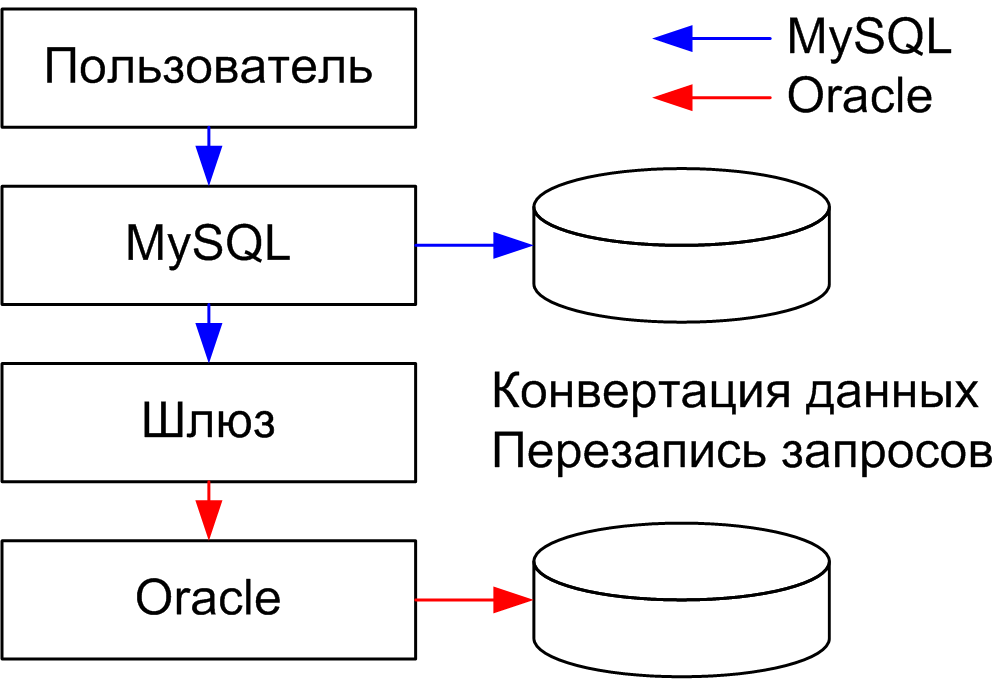
\includegraphics[width=0.8\textwidth]{../assets/kgeorgiy/distributed/Distributed_Gateway.png}
	\caption{Схема обеспечения прозрачности при использовании различных СУБД}
	\label{env-independence}
\end{figure}

Для обеспечения независимости от реализации СУБД используется механизм шлюзов, которые решают
задачи конвертации данных и перезаписи запросов. Например, Oracle предоставляет шлюз с MySQL.

Со стороны шлюх выглядит как очередная сущность СУБД. Также ожидается, что он поддерживает
распределенные транзакции и блокировки.
